%-*-coding: utf-8-*-

\chapter{Описание технических аспектов реализации}
В данной главе будут представлены технические аспекты реализации лямбд и анонимных функций.
Будет показана инженерная сложность и примененные подходы при решении поставленной задачи.

\section{Общий принцип работы}
Рассмотрим общий принцип работы \verb|KPHP| и его архитектуру и попробуем решить как правильно подходить к решению данной задачи.
\verb|KPHP| - состоит из двух основных частей:
\begin{enumerate}
\item компилятор - который занимается разбором написанного кода, построением абстрактного синтаксического дерева, анализом, трансляцией и выступает в качестве драйвера для компиляции оттранслированной программы;
\item рантайм - библиотека необходимая для запуска скомпилированных программ, содержащая скомпилированные встроенные функции языка.
\end{enumerate}

\subsection{Принцип работы компилятора}
Компилятор запускается с 24 рабочими потоками, для ускорения выполнения работ, большинство из этапов конвейера работают параллельно, что значительно уменьшает время выполнения.
На рисунке \ref{fig:compiler_arch} наглядно показана упрощенная схема основных этапов работы.
Если переход между этапами обозначен стрелочкой - это значит, что результат от предыдущего этапа сразу же передается на следующий.
Переходы же имеющие круглый конец означают, что мы должны дождаться выполнения всех предыдущих этапов во всех потоках выполнения перед тем как продолжить.

\begin{figure}[H]
    \caption{Общий принцип работы компилятора}
    \label{fig:compiler_arch}
    \centering
    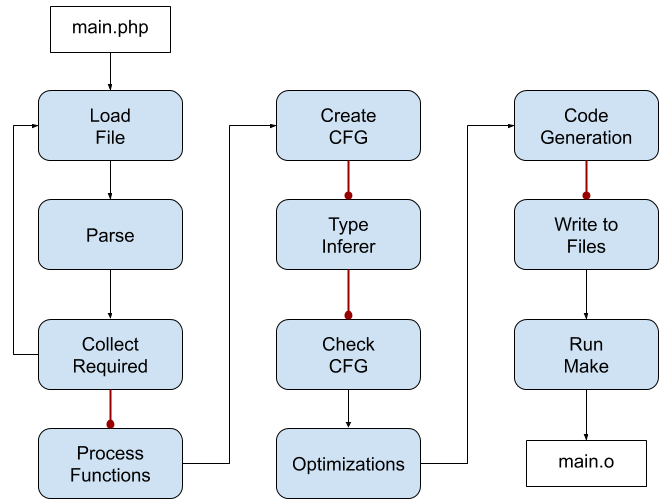
\includegraphics[width=\linewidth]{images/compiler_arch}
\end{figure}  

Помимо множества аргументов, которые передаются на вход при запуске компилятора, нас будет интересовать только один - это путь к файлу, который является отправной точкой для компиляции.
Данный файл передается в начало конвейера, на рисунке \ref{fig:compiler_arch} - это файл с именем <<\verb|main.php|>>.
На этапе <<\verb|Load File|>> мы полностью загружаем переданный нам файл в память для дальнейшего разбора и анализа.
После чего у нас происходит разбиение его на токены и построение из них абстрактного синтаксического дерева для конкретного потока символов.
Имея построенное дерево разбора мы можем понимать какие вершины у нас встречаются и без труда выявляем все зависимости, которые нам будут необходимы для дальнейшей работы. 
Каждый файл, который является зависимостью для предыдущего пришедшего файла отправляется снова на стадию <<\verb|Load File|>> и все этапы повторяются с самого начала.

На вход следующего шага нам уже передаются только разобранные функции.
При прохождении через <<\verb|Process Functions|>>  функций одна из основных задач расставить всем вершинам, соответствующим вызову другой функции, необходимые идентификаторы.
Это важный этап к которому уже должны быть разобраны все функции из других файлов, чтобы суметь проставить ссылки. Далее у нас происходит построение \verb|CFG| \cite{CFG}, необходимого для дальнейшего анализа и оптимизаций.

Вывод типов для переменных, параметров функций, а также возвращаемых значений, происходит на шаге <<\verb|Type Inferer|>>.
В этот момент компилятор использует специальный файл - <<\verb|functions.txt|>>, содержащий аннотирование встроенных функции, которые необходимы программистам на языке \verb|KPHP|.
Так как мы не имеем тела самих функций, мы вынуждены вводить свою аннотацию в этом случае.
Вывод типов в этом случае опирается на то, что написано в этом файле.
Дальше мы проверяем корректность и различные ограничения используя построенный \verb|CFG| и выведенные типы у вершин и пытаемся оптимизировать на уровне \verb|AST| наши функции.

После основных этапов мы получаем готовые деревья \verb|AST| для всех функций.
Необходимо сгенерировать их в текстовое представление для последующей записи в файлы.
Учитывая выведенные типы мы должны там где необходимо печатать соответствующие типы выражений, а также в зависимости от вида вершины преобразовать в соответствующий код на языке \verb|C++|.
Далее уже готовое текстовое представление распределенное по файлам необходимо записать на диск с нужным распределением по директориям для ускорения дальнейшей сборки.

Последний из основных этапов, который мы рассмотрим - это <<\verb|Run Make|>>.
На данном этапе мы смотрим на времена изменений файлов и понимаем какие зависимости нужно пере собрать.
Сборка происходит в несколько этапов:
\begin{enumerate}
  \item компиляция одной единицы трансляции;
  \item многопоточная линковка независимых групп бинарных файлов;
  \item линковка всех промежуточно слинкованных файлов в один исполняемый файл.
\end{enumerate}

На текущий момент мы должны уже получить исполняемый файл, который нуждается только в библиотеке с реализациями всех встроенных методов и содержащей всю необходимую функциональность для работы программы.

\subsection{Устройство рантайма}
У созданного кода компилятором, есть несколько шагов которые необходимо выполнить в рантайме для запуска.
Среда выполнения содержит в себе функцию \verb|main| с которой начинается выполнение скрипта.
Там происходит инициализация необходимых глобальных констант, которые сгенерировал компилятор.
Проставляют необходимые функции для запуска и чистки памяти, по завершении.

Также библиотека рантайма содержит все нехватающие символы для резолвинга в собранном исполняемом файле.
Они все пишутся на \verb|C++| с нужными типами указанными в файле, который мы уже встречали - <<\verb|functions.txt|>>.
Все функции начинаются с префикса \verb|f$| и имеют типы такие, какие указаны в аннотации к функции.
Если например функция принимает параметр, имеющий тип \verb|Any| - то такая функция должна иметь шаблонную сигнатуру \cite[с.~665]{Stroustrup}.

Для большинства примитивных типов участвующих в работе программы написаны соответствующие обертки.
Так например есть реализация строк, которая поддерживает необходимую COW \cite{COW} семантику и весь набор используемой функциональности, такой как: конкатенация строк, удаление подстроки, взятие конкретного символа и так далее.
Также имеется реализация \verb|PHP| массивов, которые по совместительству являются словарями.

Так как мы имеем дело с динамически типизированным языком, то у нас есть желание и право сохранять значения разных типов в одну и туже переменную.
Для этого был написан класс \verb|var|, который является типом-суммой и может содержать в себе любой из приметивных типов.
Также есть возможность превращать его обратно в строку, число, массив.
Такой класс имеет несколько проблем, связанных с производительностью, так как нам каждый раз нужно приводить его к специальному типу и проверять был ли он таковым.
Данный тип не может содержать пользовательские структуры по очень простой причине - их очень много для того, чтобы поддерживать такой тип, который мог бы хранить любой из экземпляров классов.
А создавать общий тип от которого наследовались бы все остальные классы - накладно с точки зрения производительности и потребления памяти.
Как минимум мы начнем потреблять на 8 байт больше при создании любого класса и при обращении мы будем вынуждены приводить его обратно.
Такое стало возможно при появлении интерфейсов созданных в ходе написания данной работы, но там программист явно понимает возможные недостатки при их использовании.

Все пользовательские структуры у нас хранятся отдельно в файле и представляют собой обычные \verb|C++| классы.
Методы имеющиеся в классе выносятся как глобальные функции, принимающие \verb|$this| первым параметром.
У данного подхода есть свои преимущества и недостатки.
С одной стороны это вносит небольшую неясность с первого взгляда и непонимания какие методы связаны с каким классом - в сгенерированном коде.
С другой стороны данный подход хорош тем, что все методы класса независимы и лежат в отдельных единицах трансляции, а при изменении сигнатуры одного из методов мы не будем вынуждены компилировать снова весь класс и все его методы.
Таким образом мы заключаем, что данный подход является оправданным решением в текущей архитектуре реализации пользовательских классов.

\section{Анонимные функции}
\subsection{Разбор синтаксиса}
\subsection{Вывод типов}
\subsection{Кодогенерация}

\section{Шаблонные функции}

\section{Поддержка интерфейсов}
\subsection{Разбор синтаксиса}
\subsection{Генерация методов}
\subsection{Лямбды как члены классов}

\chapterconclusion
